\documentclass[tikz]{standalone}
\usepackage{pgfplots}

\usepackage{xcolor}

\definecolor{myblue}{HTML}{367FD0}
\definecolor{myred}{HTML}{CA3F3A}

% \usepackage[showframe]{geometry}
% \geometry{
%   paperwidth=85.29mm,
%   paperheight=51mm,
%   margin=0mm,
% }
\begin{document}
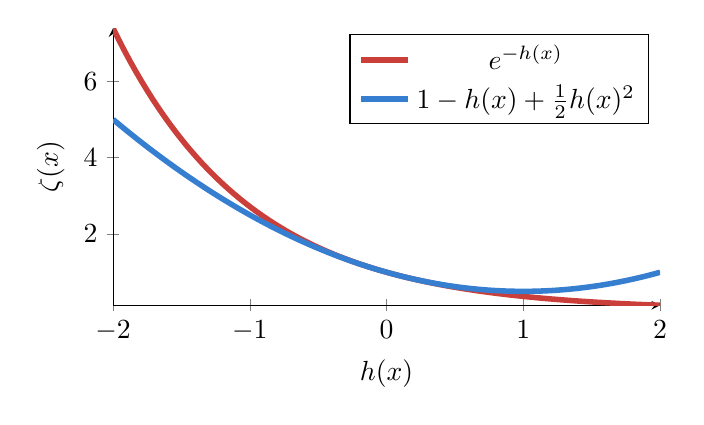
\begin{tikzpicture}
\begin{axis}[
  width=85.29mm,
  height=51mm,
  axis lines = left,
  xlabel = \(h(x)\),
  ylabel = {\(\zeta(x)\)},
  ]
  % Negative Exponential
  \addplot [line width=2pt, domain=-2:2, samples=100, color=myred]{e^(-x)};
  \addlegendentry{\(e^{-h(x)}\)}
  % Taylor Approx
  \addplot [line width=2pt, domain=-2:2, samples=100, color=myblue]{1 - x + (x^2)/2};
  \addlegendentry{\(1 - h(x) + \frac{1}{2}h(x)^2\)}
\end{axis}
\end{tikzpicture}
\end{document}
%%% Local Variables:
%%% mode: latex
%%% TeX-master: t
%%% End:

